\section{Case Study: Interconnect Resource Sharing} \label{sec:case_study_1042}

\begin{figure}[!htbp]
\begin{center}
\begin{subfigure}[b]{\linewidth}
  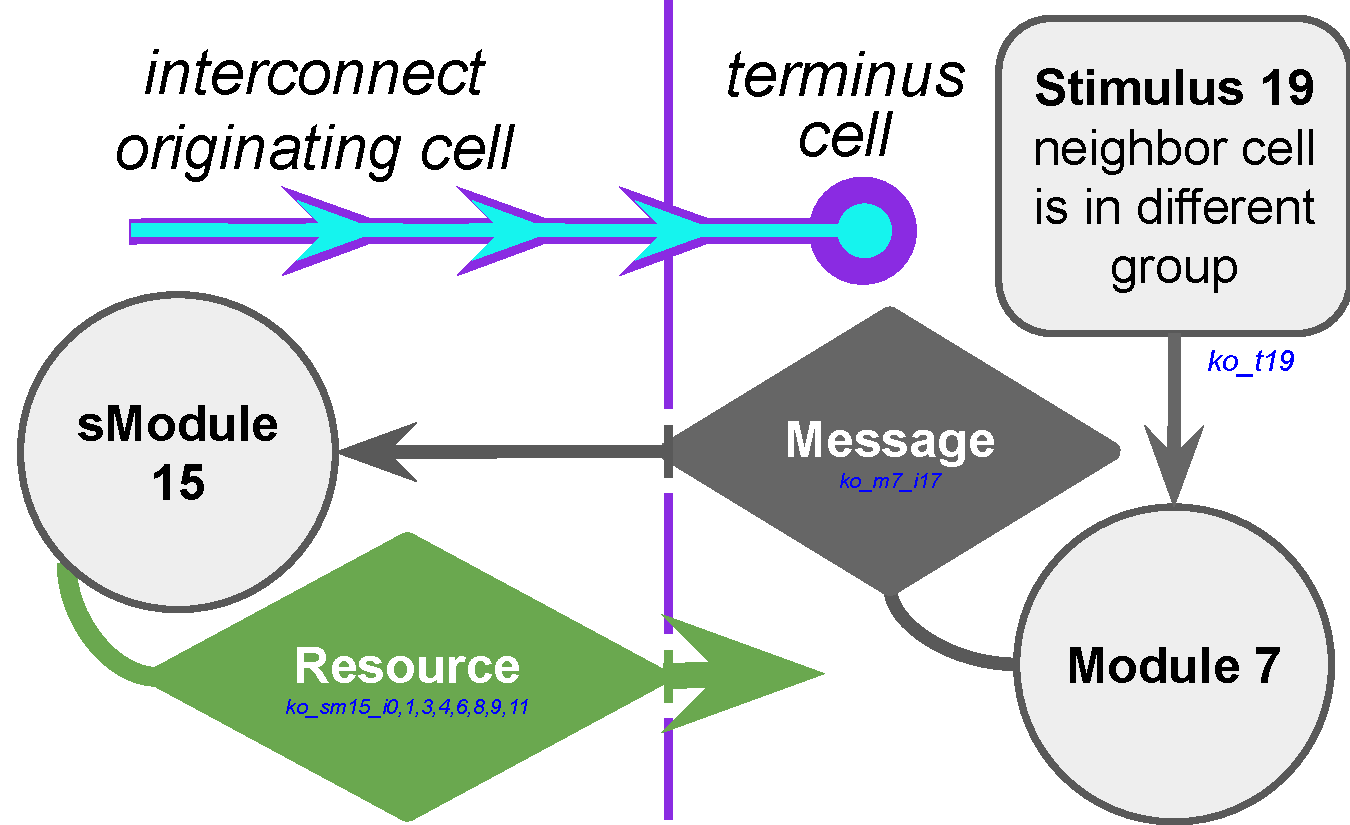
\includegraphics[width=\linewidth,clip]{batch=1042+step=1024+pop=3/1042_diagram}
  \caption{TODO}
  \label{fig:TODO}
\end{subfigure}
\begin{subfigure}[b]{0.33\linewidth}

  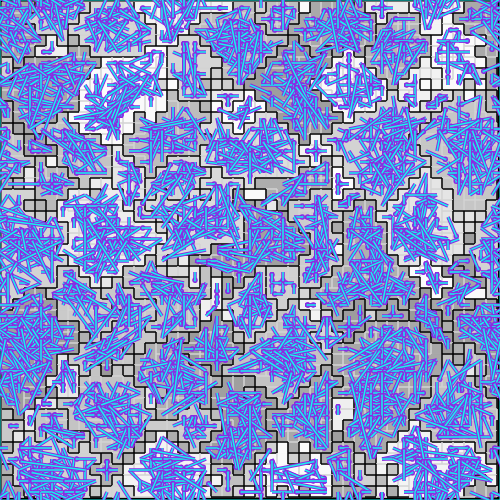
\includegraphics[width=\linewidth,trim={0 100 100 0},clip]{batch=1042+step=1024+pop=3/seed=1+title=established-interconnect+treat=batch_1042,step_1024,pop_3,id1_wt+update=4990+_emp_hash=0c549f0-clean+_source_hash=a6072a6-clean+ext=}
  \caption{TODO}
  \label{fig:TODO}
\end{subfigure}
\begin{subfigure}[b]{0.33\linewidth}
  
\includegraphics[width=\linewidth,trim={0 100 100 0},clip]{batch=1042+step=1024+pop=3/seed=1+title=channel+treat=batch_1042,step_1024,pop_3,id1_wt+update=4990+_emp_hash=0c549f0-clean+_source_hash=a6072a6-clean+ext=}
  \caption{TODO}
  \label{fig:TODO}
\end{subfigure}
\begin{subfigure}[b]{0.33\linewidth}
  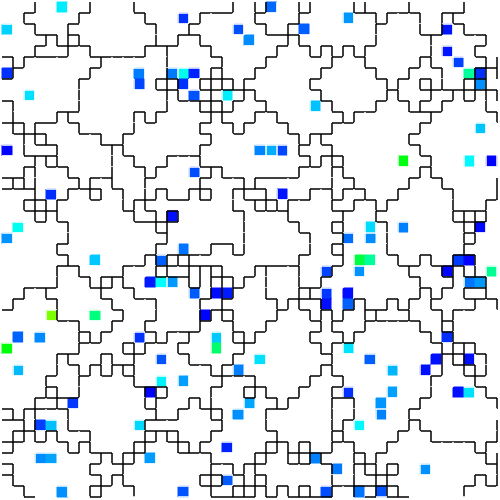
\includegraphics[width=\linewidth,trim={0 100 100 0},clip]{batch=1042+step=1024+pop=3/seed=1+title=interconnect-shared-resource+treat=batch_1042,step_1024,pop_3,id1_wt+update=4990+_emp_hash=0c549f0-clean+_source_hash=a6072a6-clean+ext=}
  \caption{TODO}
  \label{fig:TODO}
\end{subfigure}
\begin{subfigure}[b]{0.33\linewidth}
  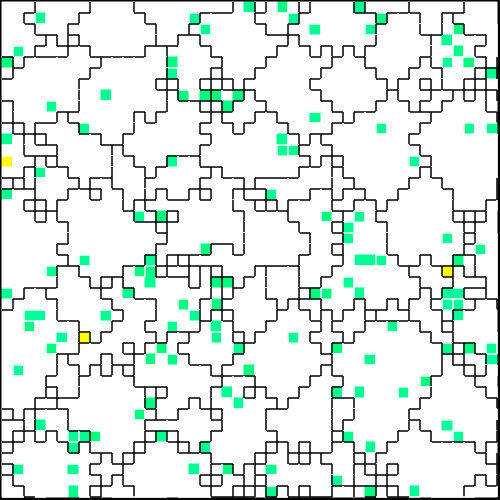
\includegraphics[width=\linewidth,trim={0 100 100 0},clip]{batch=1042+step=1024+pop=3/seed=1+title=interconnect-sharing-fraction+treat=batch_1042,step_1024,pop_3,id1_wt+update=4990+_emp_hash=0c549f0-clean+_source_hash=a6072a6-clean+ext=}
  \caption{TODO}
  \label{fig:TODO}
\end{subfigure}
\caption{
TODO
}
\label{fig:case_study_1042}
\end{center}
\end{figure}


This case study was drawn from epoch 24 of batch 42 of the initial set of evolutionary runs.
We initially considered it for further study due to the presence of widespread over-interconnect resource sharing.
After preliminary knockout experiments confirmed the adaptive significance of both over-interconnect resource-sharing and over-interconnect messaging, we set aside the strain for a case study.
The evolutionary history preceding this case study consumed approximately 96 hours of wall-clock time and 736 compute-core hours.
Approximately 30 million simulation updates and 40,000 cellular generations elapsed.
You can view the strain this case study characterizes in a live in-browser simulation at \url{https://mmore500.com/hopto/8}

% 100%|████████████████████████████████████████████████████████████████████████████████████████████████████████████████████████████████████████| 25/25 [00:00<00:00, 292.67it/s]
% Output saved to title=mastergenerations+_data_hathash_hash=dc05faa593102bf1+_script_fullcat_hash=5e6b7a64514cbb09+_source_hash=aa98eba-clean+ext=.csv
% level 0
% Generations Elapsed mean 41438.728819430224
% Generations Elapsed std nan
% Generations Elapsed min 41438.728819430224
% Generations Elapsed max 41438.728819430224
% level 1
% Generations Elapsed mean 24466.75578134247
% Generations Elapsed std nan
% Generations Elapsed min 24466.75578134247
% Generations Elapsed max 24466.75578134247
% level 2
% Generations Elapsed mean 5130.206547616208
% Generations Elapsed std nan
% Generations Elapsed min 5130.206547616208
% Generations Elapsed max 5130.206547616208

% EXPIRATION_UPDATE 361120
% EXPIRATION_UPDATE 336640
% EXPIRATION_UPDATE 439872
% EXPIRATION_UPDATE 247360
% EXPIRATION_UPDATE 255456
% EXPIRATION_UPDATE 239904
% EXPIRATION_UPDATE 230144
% EXPIRATION_UPDATE 119168
% EXPIRATION_UPDATE 232736
% EXPIRATION_UPDATE 238400
% EXPIRATION_UPDATE 270912
% EXPIRATION_UPDATE 125856
% EXPIRATION_UPDATE 204256
% EXPIRATION_UPDATE 242368
% EXPIRATION_UPDATE 190432
% EXPIRATION_UPDATE 270880
% EXPIRATION_UPDATE 244544
% EXPIRATION_UPDATE 216064
% EXPIRATION_UPDATE 282688
% EXPIRATION_UPDATE 254048
% EXPIRATION_UPDATE 309120
% EXPIRATION_UPDATE 279904
% EXPIRATION_UPDATE 342848
% EXPIRATION_UPDATE 289248
% EXPIRATION_UPDATE 237664
% EXPIRATION_UPDATE 166016
% EXPIRATION_UPDATE 251520
% EXPIRATION_UPDATE 207424
% EXPIRATION_UPDATE 260064
% EXPIRATION_UPDATE 248480
% EXPIRATION_UPDATE 301312
% EXPIRATION_UPDATE 225088
% EXPIRATION_UPDATE 347072
% EXPIRATION_UPDATE 321120
% EXPIRATION_UPDATE 344448
% EXPIRATION_UPDATE 388256
% EXPIRATION_UPDATE 382336
% EXPIRATION_UPDATE 454560
% EXPIRATION_UPDATE 413312
% EXPIRATION_UPDATE 404512
% EXPIRATION_UPDATE 437920
% EXPIRATION_UPDATE 402560
% EXPIRATION_UPDATE 435552
% EXPIRATION_UPDATE 420384
% EXPIRATION_UPDATE 366752
% EXPIRATION_UPDATE 401440
% EXPIRATION_UPDATE 318752
% EXPIRATION_UPDATE 395936
% EXPIRATION_UPDATE 176608
% EXPIRATION_UPDATE 194656
% EXPIRATION_UPDATE 228928
% EXPIRATION_UPDATE 115776
% EXPIRATION_UPDATE 272000
% EXPIRATION_UPDATE 282176
% EXPIRATION_UPDATE 223232
% EXPIRATION_UPDATE 176320
% EXPIRATION_UPDATE 334080
% EXPIRATION_UPDATE 359328
% EXPIRATION_UPDATE 404000
% EXPIRATION_UPDATE 277824
% EXPIRATION_UPDATE 206592
% EXPIRATION_UPDATE 189024
% EXPIRATION_UPDATE 216736
% EXPIRATION_UPDATE 166624
% EXPIRATION_UPDATE 194560
% EXPIRATION_UPDATE 198336
% EXPIRATION_UPDATE 182080
% EXPIRATION_UPDATE 173824
% EXPIRATION_UPDATE 309440
% EXPIRATION_UPDATE 281888
% EXPIRATION_UPDATE 345280
% EXPIRATION_UPDATE 326144
% EXPIRATION_UPDATE 259680
% EXPIRATION_UPDATE 292096
% EXPIRATION_UPDATE 205056
% EXPIRATION_UPDATE 216672
% EXPIRATION_UPDATE 355360
% EXPIRATION_UPDATE 401824
% EXPIRATION_UPDATE 388768
% EXPIRATION_UPDATE 434080
% EXPIRATION_UPDATE 280480
% EXPIRATION_UPDATE 307104
% EXPIRATION_UPDATE 350592
% EXPIRATION_UPDATE 279424
% EXPIRATION_UPDATE 424000
% EXPIRATION_UPDATE 404160
% EXPIRATION_UPDATE 412640
% EXPIRATION_UPDATE 376768
% EXPIRATION_UPDATE 325216
% EXPIRATION_UPDATE 366816
% EXPIRATION_UPDATE 380384
% EXPIRATION_UPDATE 361664
% EXPIRATION_UPDATE 371488
% EXPIRATION_UPDATE 398400
% EXPIRATION_UPDATE 374816
% EXPIRATION_UPDATE 368416
% EXPIRATION_UPDATE 329600
% EXPIRATION_UPDATE 302016
% EXPIRATION_UPDATE 328832
% EXPIRATION_UPDATE 384832


Our first step was to evaluate whether the intercellular nature of over-interconnect messaging and resource sharing contributed to this strain's fitness.
(It is possible that messaging and/or resource sharing behaviors might generate stimuli on the recipient or side-effects on the sender that have adaptive consequences whether or not the sender and recipient are distinct cells;
in such a scenario, cells would be just as well off sending messages and/or resource to themselves.)
We performed several competition experiments between between the wild-type strain and variants where interconnect messaging and resource sharing was altered to be intracellular instead of intercellular.
At the end of competition experiments, we evaluated the relative abundances of wild-type and variant strains.
In the first variant strain we tested, all outgoing over-interconnect messages were instead delivered to the sending cell.
In 16 out of 16 one-hour competition runs that were seeded half-and-half with the wild-type and variant strains, the wild-type strain drove the variant strain to extinction (one-tailed binomial test; $p < 0.0001$; 290 S.D 17 cell gens elapsed).
We observed a similar outcome with a second variant strain where all outgoing over-interconnect resource sharing was rerouted back to the sending cell (14/16 variant strain extinctions; 16/16 wild-type prevalence; 289 S.D. 25 cell gens elapsed).
Finally, a third variant strain where both over-interconnect messaging and over-interconnect resource sharing were returned to the sending cell exhibited the same outcome (16/16 variant strain extinctions; 300 S.D. 23 cell gens elapsed).
The intercellular natures of both over-interconnect messaging and resource sharing appear essential to fitness.

Next, we took a closer look at the evolved cellular mechanisms controlling over-interconnect messaging and resource sharing.
We monitored hardware execution of the wild-type strain in a monoculture population to detect which signals, messages, and fork/call instructions activated each SignalGP module.
We manually cross-referenced this information with a human-readable printout of the strain's genetic program to construct a hypothesized mechanism shown in Figure \ref{fig:case_study_1042}.
We hypothesize that cells at the periphery of a registered kin groups send messages backwards over incoming interconnects that induce interconnect-originating cells to send them resource.
Such a mechanism could preferentially increase resource availability at the group periphery, a region where cell-cell conflict is likely elevated.

We performed a series of four-hour competition experiments between wild type and knockout strains to confirm the adaptive significance of each component of this mechanism.
We began by re-routing stimulus 19, which alerts cells to neighbors that are members of a foreign kin group, to activate a known no-op module.
This knockout strain experienced decreased fitness compared to the wild-type strain (16/16 knockout strain extinctions; one-tailed binomial test; $p < 0.0001$; 1996 S.D. 280 cell gens elapsed; \url{https://mmore500.com/hopto/ak}).
Next, we replaced the over-interconnect messaging instruction that triggers over-interconnect resource-sharing with a no-op instruction.
This knockout strain also experienced decreased fitness (16/16 knockout strain extinctions; 1932 S.D. 223 cell gens elapsed; \url{https://mmore500.com/hopto/al}).
We then replaced all eight copies of the over-interconnect resource-sharing instruction triggered by the over-interconnect messaging with no-op instructions, once more yielding a strain with diminished fitness (16/16 knockout strain extinctions; 1860 S.D. 370 cell gens elapsed; \url{https://mmore500.com/hopto/am}).
Finally, we confirmed the soundness of our fitness competition methodology by running control wild-type versus wild-type competitions.
As expected, we observed no effect of strain ID on competition dominance (8/16 knockout strain extinctions; 8/16 wild-type strain extinctions; one-tailed binomial test; $p = 0.60$; 1738 S.D. 217 cell gens elapsed; \url{https://mmore500.com/hopto/aj})

